\section{Implementation}
We have implemented the lens synthesis algorithm in $n$ lines of OCaml code.

\subsection{Synthesis Overview}
\begin{figure}
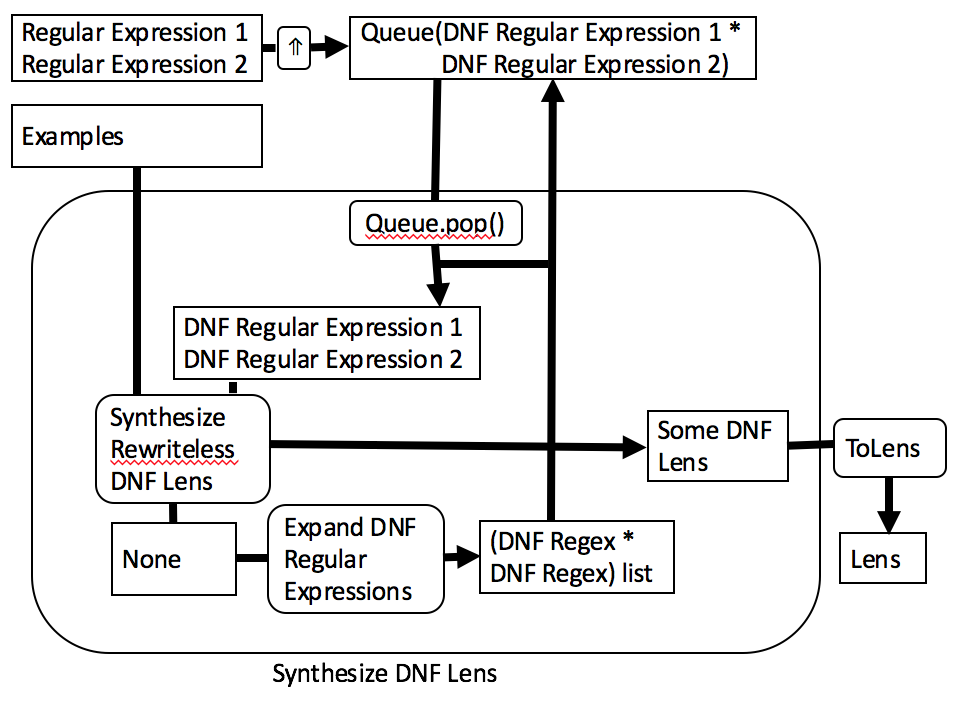
\includegraphics[scale=.5]{synth-lens-schematic.png}
\label{fig:synth-lens-schematic}
\end{figure}
The synthesis algorithm is shown in a schematic diagram in 
Figure~\ref{fig:synth-lens-schematic}.  The algorithm takes in a pair of
regular expressions, and examples, and converts the regular expressions into
DNF regular expressions, using \ToDNFRegex{}.
These then get enqueued, and SynthDNFLens, where the bulk of the work
occurs.

In SynthDNFLens, the highest priority DNF regular expression pair is popped.
Then, SynthRewritelessDNF sees if a DNF lens which satisfies the examples, which
does not include any applications of the rewrite rule, can be found.
If none are found, then each rewrite is applied once on each side of the regular
expressions.
This new list of DNF regular expression doubles is enqueued, and SynthDNFLens is
called again.
If one is found, this DNF lens gets converted to a normal lens, and is returned
to the user.

\subsection{Priority Queue}
The priority queue is implemented with a list implementation of a priority queue.
We say that the lower the priority value, the higher the priority.
The priority value of an element is based on the number of expansions that have been
preformed, combined with the distance between the two regular expressions, based
on a psuedometric $\Distance$ we have implemented.  This pseudometric is implemented
as the sum of simpler pseudometrics,
$\Distance = \Distance_{size}+\Distance_{dist}$.

$\Distance_{size}$ is defined as merely the difference in the sizes of the DNF
regular expressions.
$\Distance_{size}(\DNFRegex,\DNFRegexAlt)=\AbsOf{\Size(\DNFRegex)-\Size(\DNFRegexAlt)}$

$\Distance_{dist}$ captures how far apart the distribution of
user defined regular expressions are.
The distribution of user defined regular expressions can be viewed as an
infinite dimensional free module over the integers, \Module{}.
The basis for this is $\SetOf{1*(\RegexVariable,n) | n\in\Nats, \RegexVariable
\text{ is a user defined regular expression}}$
DNF regular expressions with variables can map into this with a function by
counting the number of user defined data types present at a given level.
The formal definition for this mapping is given by the function \GetDist{}.

\begin{definition}\leavevmode\\
\label{def:getdist}
\begin{tabular}{@{}L@{}L@{}}
\GetDist(\DNFOf{\Sequence_1;\ldots;\Sequence_n}) &
=\GetDist(\Sequence_1)+\ldots+\GetDist(\Sequence_n)\\
\GetDist(\SequenceOf{\String_0;\Atom_1;\ldots;\Atom_n;\String_n}) &
=\GetDist(\Atom_1)+\ldots+\GetDist(\Atom_n)\\
\GetDist(\RegexVariable)&=1*(\RegexVariable,1)\\
\GetDist(\IterateLens{\DNFLens})&=\phi(\GetDist(\DNFLens))
\end{tabular}

where $\phi$ is the linear map sending $1*(\RegexVariable,n)$ to
$1*(\RegexVariable,n+1)$
\end{definition}

Using this, we now have a mapping from regular expressions into the distribution
of user defined regular exprssions.

$\Distance_{dist}(\DNFRegex,\DNFRegexAlt)=\LOneNorm(\phi(\DNFRegex),\phi(\DNFRegexAlt))$
where \LOneNorm{} is the taxicab metric on \Module{}.
The priority of a pair of DNF regular expressions, $(\DNFRegex{},\DNFRegexAlt{})$,
is $\Distance(\DNFRegex{},\DNFRegexAlt{})+8*expansion_{count}$.
Keeping track of expansion count is important as it allows for lower priority
expansions to be eventually popped, instead of getting stuck doing incorrect,
increasingly deep expansions whose DNF regular expressions have a low distance.
\afm{should i do an example, or is that going into too much detail?}
Experimentally, 8 was a good value for how much weight the expansion
count should get in the priority.  It allows for not getting stuck in a local
minima in the search space, while still allowing for the distance to choose the
correct expansion the majority of the time.

\subsection{SynthRewritelessDNF}
We find an efficient way to synthesize DNF lenses which do not use rewrites
through a clever encoding of the DNF regular expressions and examples.
A key insight into efficiently finding DNF lenses between two DNF regular
expressions is finding an ordering of DNF regular expressions which satisfy the
property such that, for two regular expressions $\DNFRegex$ and $\DNFRegexAlt$,
$\DNFRegex \leq \DNFRegexAlt$ and $\DNFRegexAlt \leq \DNFRegex$ if, and only if,
for some dnf lens $\DNFLens \OfType \DNFRegex \Leftrightarrow \DNFRegexAlt$,
with no use of \DNFRewriteLensRule{}.

ATTEMPT TO WRITE IT LESS FORMALLY

Unfortunately, while synthesizing a DNF regular expression, we must synthesize
two permutations, one to deal with determining which sequence
gets mapped to which (handling the commutativity of +), and one to deal
with determining within a sequence, which atoms get mapped to which
(handling swaps).

We found an incredibly efficient strategy for doing this, by further normalizing
the DNF regular expressions.  Instead of allowing any order of sequences, we
provide a total preorder on sequences, and order order the sequences
according to that ordering.

We do the same trick for normalizing the sequences.  While reordering a sequence
changes the semantics, we can temporarily reorder the sequence, remembering the
permutation of the reordering, and recover the original sequence later.

\begin{definition}
Given an ordering $\leq : A \rightarrow A \rightarrow \SetOf{-1,0,1}$,
we denote the dictionary ordering on lists of $As$, $\ListOf{\leq}$.
\end{definition}

\begin{definition}
  Given an ordering $\leq : A \rightarrow A \rightarrow \SetOf{-1,0,1}$,
  and $\ListOf{a_1;\ldots;a_n}\in A \ListType$
  We define $\SortingOf{\leq}{\ListOf{a_1;\ldots;a_n}}$ as
  $\sigma \in \PermutationSetOf{n}$ where if $i\leq j$,
  then $a_{\sigma(i)} \leq a_{\sigma(j)}$.

  We define $\SortOf{\leq}{\ListOf{a_1;\ldots;a_n}}$ as
  $\ListOf{a_{\sigma(1)};\ldots;a_{\sigma(n)}}$ where
  $\sigma=\SortingOf{\leq}{\ListOf{a_1;\ldots;a_n}}$
\end{definition}

\begin{definition}
  \begin{enumerate}
  \item
    $\DNFOf{\Sequence_1;\ldots\Sequence_n}
    \DNFLeq
    \DNFOf{\SequenceAlt_1;\ldots\SequenceAlt_m}$
    if
    $\SortOf{\SequenceLeq}{\ListOf{\Sequence_1;\ldots;\Sequence_n}}
    \ListOf{\SequenceLeq}
    \SortOf{\SequenceLeq}{[\SequenceAlt_1;\ldots;\SequenceAlt_n]}$.
    
  \item
    $\SequenceOf{\String_0;\Atom_1;\ldots;\Atom_n;\String_n}
    \SequenceLeq
    \SequenceOf{\StringAlt_0;\AtomAlt_1;\ldots;\AtomAlt_n;\String_n}$
    if
    $\SortOf{\AtomLeq}{\ListOf{\Atom_1\ldots\Atom_n}}
    \ListOf{\AtomLeq}
    \SortOf{\AtomLeq}{[\AtomAlt_1\ldots\AtomAlt_n]}$.

  \item
    $\StarOf{\DNFRegex} \AtomLeq \StarOf{\DNFRegexAlt}$
    if
    $\DNFRegex \DNFLeq \DNFRegexAlt$
  \end{enumerate}
\end{definition}

This allows us to put our DNF regular expressions into a more normal form.

\begin{definition}
  \begin{enumerate}
  \item A DNF regular expression $\DNFOf{Sequence_1;\ldots;\Sequence_n}$ is
    \textit{normalized} if $i \leq j$ implies $\Sequence_1\SequenceLeq\Sequence_j$,
    and each $\Sequence_i$ is normalized.
  \item A sequence $\SequenceOf{\Atom_1;\ldots;\Atom_n}$ is \textit{normalized}
    if $i \leq j$ implies $\Atom_i\AtomLeq\Atom_j$,
    and each $\Atom_i$ is normalized.
  \item An atom $\StarOf{\DNFRegex}$ is \textit{normalized} if
    $\DNFRegex$ is normalized.
  \end{enumerate}
\end{definition}

We can also easily normalize a DNF regular expression

\begin{definition}
  \begin{enumerate}
  \item $\NormalizeOf{\DNFOf{\Sequence_1;\ldots;\Sequence_n}} =
    \DNFOf{\NormalizeOf{\Sequence_{\sigma(1)}};\ldots;\NormalizeOf{\Sequence_{\sigma(n)}}}$,
    where
    $\sigma=\SortingOf{\SequenceLeq}
    {\ListOf{\NormalizeOf{\Sequence_1};\ldots;\NormalizeOf{\Sequence_n}}}$
  \item $\NormalizeOf{\SequenceOf{\String_0;\Atom_1;\ldots;\Atom_n;\String_n}} =
    \SequenceOf{\String_0;\Atom_{\sigma(1)};\ldots;\Atom_{\sigma(n)};\String_n}$,
    where
    $\sigma=\SortingOf{\SequenceLeq}
    {\ListOf{\NormalizeOf{\Atom_1};\ldots;\NormalizeOf{\Atom_n}}}$
  \item $\NormalizeOf{\StarOf{\DNFRegex}}=\StarOf{\NormalizeOf{\DNFRegex}}$
  \end{enumerate}
\end{definition}

Critically, the normalized form of the DNF regular expression, and the ordering
on DNF regular expressions, are tied to the existance of a DNF Lens without
rewrites.

\begin{theorem}
  $\NormalizeOf{\DNFRegex}\DNFLeq\NormalizeOf{\DNFRegexAlt}$ and
  $\NormalizeOf{\DNFRegexAlt}\DNFLeq\NormalizeOf{\DNFRegex}$ if, and only
  if, there exists a $\DNFLens \OfType \DNFRegex \Leftrightarrow \DNFRegexAlt$,
  where $\DNFLens$ has no applications of a rewrite rule.
\end{theorem}

This can be proven with mutual induction, proving similar statements for
sequences and atoms.

Furthermore, two DNF regular expressions can be zipped together to form a
DNF lens.  Consider $\DNFOf{\Sequence_{\sigma_1(0)};\ldots;\Sequence_{\sigma_1(n)}}$, and
$\DNFOf{\SequenceAlt_{\sigma_2(0)};\ldots;\SequenceAlt_{\sigma_2(n)}}$, two normalized
DNF regular expressions.  $\Sequence_{\sigma(0)}$ merely needs to be mapped to
$\SequenceAlt_{\tau(0)}$.  Furthermore, the permutation mapping the two lenses
merely needs to be $\sigma_1 \Compose \sigma_2^{-1}$

We can use these orderings to find 

Beyond that, we can use these orderings to find the lenses.
If $\DNFOf{\Sequence_1;\ldots;\Sequence_n}\leq\DNFOf{\SequenceAlt_1;\ldots;\SequenceAlt_n}$,
and $\DNFOf{\SequenceAlt_1;\ldots;\SequenceAlt_n}\leq\DNFOf{\Sequence_1;\ldots;\Sequence_n}$,
then $\Sorting([\Sequence_1;\ldots;\Sequence_n])\leq\Sorting([\Sequence_1;\ldots;\Sequence_n])$
using the dictionary ordering, which means that
$\Sorting([\Sequence_1;\ldots;\Sequence_n])[i]\leq
\Sorting([\SequenceAlt_1;\ldots;\SequenceAlt_n])[i]$ and
$\Sorting([\SequenceAlt_1;\ldots;\SequenceAlt_n])[i]\leq
\Sorting([\Sequence_1;\ldots;\Sequence_n])[i]$, which means that there is a
sequence lens between them.
\afm{I can keep going on about this stuff, should it go here?  Should I just make a brief claim
about it and move on}

Unfortunately, while this can find a well typed DNF regular expression, it doesn't
necessarily find the one that matches the examples.  In the situation where
there are multiple valid sorted orderings, there are multiple different lenses
with potentially different semantics.  Instead of iterating through all the
possible sortings, and finding one that matches the examples, we would like to
be able to immediately find only a sorting which satisfies the examples.

The key insight here is that certain invariants must hold for a DNF lens to have
semantics which match the examples.

\begin{enumerate}
\item If a source example string matches one of the clauses during parsing,
it must be sent to the clause the target example string matches during parsing.
\item If a source example string matches a user defined regular expression during
parsing, the target must match the exact same string during parsing.
\item If a source example string matches an iteration, then the target must iterate
the same number of times, and all the invariants must hold for each iterated part.
\end{enumerate}

This is done by joining additional parsing information alongside the regular
expression components.

%%% Local Variables:
%%% TeX-master: "main"
%%% End: